\section{Multi-round Batch Scheduling}
\label{sect:scheduling}
The naive way for synchronized backup is   to schedule all of the backup tasks in one round.
Since parallel backup of these tasks goes through several stages,
that results in the backup time of each VM is approximately equal to the total execution of all backup tasks.
Given VM sizes are highly skewed in a large cluster, some big VMs will take a long time and other
small VM backup tasks synchronized in one round will have to wait.
Thus the average backup time for small VMs is fairly large. 

%Figure~\ref{sizeDistribution} shows the size distribution of VMs for a dataset from Alibaba containing
%about 3000VMs. The largest VM size is to a few terabytes while  the smallest VMs only have a few gigabytes of data.
%The percentage of changes from last backup is also show in the graph and 
%it shows that the change is fairly uniform for large VMs also. Namely when scheduling all VM backup tasks
%in one round in a synchronized manner, and the average backup time per VM is fairly large.

There is another disadvantage with a single-round scheduling. 
During backup period, new data modification requests can lead a inconsistency between data signature 
read previously and actual data on the disk.
% This works well if all of the
% data being backed up are only copies, e.g. a separate backup system which data
% is sent to over the network. 


%However, in our case we are backing up the
%live virtual disks, thus such single round backup presents several problems
%in our synchronous approach.
In order to preserve a consistent view of VM images, we employ
the Copy-on-Write (CoW) technique to protect the dirty segments against incoming disk writes during 
the backup period~\cite{VMare2013}. 
The cost of CoW is a factor of the data size, the write rate, and duration of CoW protection.
Previous studies have shown that as much as 8\% or even more of total disk capacity may have to be 
reserved for CoW~\cite{EMCIncrementalDataChanges}.
Prolonging the backup time of individual VM backup  caused by skewed VM size distribution
and single-round operation synchronization significantly increases COW overhead.
%The second problem is that a single round backup brings the highest cost of CoW
%because of the workload in stage 1a is imbalanced,
%causing machines with small VMs to wait while CoW protection is turned on.
%Thus we must minimize the duration that a given VM is undergoing CoW protection.

To determine how evenly distributed VM sizes are, we obtained statistical data
for 22 Aliyun clusters. The clusters in our dataset all have a very long tail distribution,
Though local minima exist in the histogram and the range of VM sizes varies. Other production clusters
may have different distributions, but our findings justify our architecture for a multi-round algorithm.
A representative histogram for one of the clusters is shown in Fig.~\ref{fig:hist-1}. You can see that the range of sizes is very large (the smallest group of 100 VMs has an average size of ~15GB, while the largest has an average size of over 700GB). It is that fact that VM sizes vary greatly that makes the scheduling of VMs to rounds important.

\begin{figure}[ht]
  \centering
  \begin{tikzpicture}
      \begin{axis}[
              ybar interval,
              xlabel=Avg VM Size in Group (GB),
              ylabel=Number of Groups,
              xticklabel={\pgfmathparse{(\tick*1)}\num[round-mode=places, round-precision=0]{\pgfmathresult}}
      ]
          \addplot+[hist={bins=10}] table[y=AY41G] {figures/cluster_distributions.txt};
      \end{axis}
  \end{tikzpicture}
  \caption{Histogram of average data sizes for a real cluster. TODO:adjust this using the new spreadsheets}
  \label{fig:hist-1}
\end{figure}


% The first is that the average turnaround time for a VM is the time it takes to
% backup all the VMs. The second, which is related to the first, is that a single
% round backup has the highest cost to maintain a consistent view of the virtual
% disks. We use Copy on Write (CoW) for this, and the consistent view must be
% maintained between stage 1a and stage 2b, which can have significant cost if
% the system must wait for every single VM before unlocking any of the VMs.
% Other studies have shown that as much as 8\% or even more of total capacity must be reserved for
% CoW \cite{EMCIncrementalDataChanges}. The actual cost of CoW is a factor of the
% data size, the write rate, and duration CoW is taking place. The data size
% isn't something we can change, nor the write rate, but we can minimize the
% duration that a given VM is undergoing CoW. By minimizing the backup time for
% individual VMs we also improve CoW cost. 

\comments{
To evaluate our CoW cost, we assume the incoming writes point to random disk locations, 
which would incur a CoW operation over a segment if the write location fall into a dirty segment
for the first time (consequential writes to that segment will be re-directed 
to the new copy so there's no extra cost). Therefore the number of dirty segments needs to be copied represents
the CoW cost of a VM.


Let $t$ be the time that a VM is under Cow protection, $w$ be the write rate
during that period, $n$ be the total number of segments and $d_1$ 
be the percentage of clean segments that don't need to
be protected, then the total number of dirty segments is
\[
n_d=n(1-d_1)
\]
and the total number of writes fall into dirty segments is
\[
w_d=tw(1-d_1)
\]
Then the total number of dirty segments that need to be copied is:
\[
Cost = n_d(1-e^{-w_d/n_d}) = n(1-d_1)(1-e^{-tw/n})
\]
From the above formula it is clear that decreasing CoW time $t$ will
reduce the CoW protection cost, 
the model we derive is similar to the results measured by \cite{EMCIncrementalDataChanges}.
% Our basic CoW cost model is:
% \[
%     CoW=n(1-e^{-m/n})
% \]
%     where
% \[
%     m=tw(1-d_1)c
% \]

% In the above model, $n$ is the number of dirty segments, $t$ is the time under
% CoW protection, $w$ is the
% write rate during CoW, $d_1$ is the \% of clean data (which doesn't go under
% CoW), and $c$ is a constant determining how likely writes are to touch dirty
% segments which haven't yet been copied vs. dirty segments which have already
% been copied during the current backup. With this CoW cost model and the earlier
% performance model, we can estimate the CoW cost of a given backup schedule.
% Note that CoW ends in Stage 2b, so only the time up to the end of 2b counts
% towards CoW. \todo{we still need to pick a value for $c$}
}

\subsection{Cost Functions and Optimization Objectives}


When a multi-round schedule is deployed, the backup of a  VM can be executed in one of these rounds.
Tasks at each round go through the processing stages discussed in Section~\ref{processingStage}.
\begin{figure}[thb]
\centering
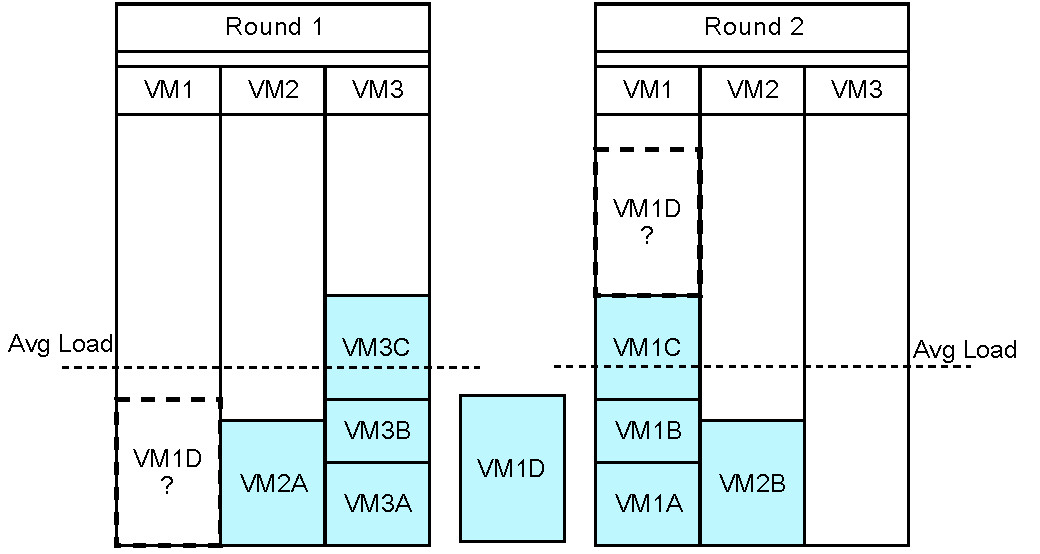
\includegraphics[width=0.5\textwidth]{images/VMRound.pdf}
\caption{Choosing a round to schedule a VM (marked as VM1D in a two-round schedule.  }
\label{fig:VMRound}
\end{figure}

The question is which round a VM backup task should be scheduled?
Figure~\ref{fig:VMRound} illustrates an intermediate step of scheduling in which
some of VMs have been assigned to a round, and they are marked with the gray boxes. 
VM named  VM1D is to be scheduled and  can be assigned  to Round 1 or Round 2.
Scheduling VM1D on Round 1 would not significantly increase the execution time of round 1
because machine M1 does not have any VM scheduled.

The disadvantage of having many rounds of backup is that the time for  the entire
backup job for all VMs is stretched for many iterations.
We call this time as the backup job span.
In practice, we would like the job span to be controlled within few hours during
night time. Thus there is a tradeoff to strike in the design of scheduling and
the optimization  metrics are listed as follow.
\begin{itemize}
\item {\em Average backup time T}.
This is to measure the average number of the backup time time. 
A smaller number will also shorten the COW cost as discussed above.
The average backup time also reflects the average computing resource required.
A shorter backup time means that the computer system devotes less resource in the backup of each VM. 
\item {\em The job span: J}.
This is to measure the total time needed to complete all backup tasks.
Longer the job span is, the more burden is imposed to the cluster management.
While a short span is better, the  constraint is not high as long as the job can be completed
in a short period of time (e.g. a few hours during night time). 

%It is generally preferred to run backups
%during low demand hours to make use of otherwise unused time and minimize the
%impact on users. This leaves a window of several hours (e.g. from 1am to 4am)
%to complete the backup. The more 
%are the shorter each round can be and therefore the smaller the VM backup times
%and the total CoW costs. The
%more rounds there are however the greater the overheads and some of the
%efficiency gained from batch processing is lessened. We balance these costs by
%developing an algorithm to schedule VMs into rounds.
\item {\em Aggregated optimization}.
We will use the following combined cost function to set the optimization objective.
\[
\alpha T + (1-\alpha) J
\]
where $\alpha$ varying between 0 and 1 represents the importance of the average backup time.
\end{itemize}

%Our round packing heuristic uses a descending sorted order worst fit packing, 
%Scheduling VMs machine by machine, and is described in Fig~\ref{fig-bpl}.
%For our higher-level scheduling algorithm, we minimize Resource usage and average
%backup time, while ensuring that the jobspan constaint is met (if possible). The
%overall scheduling algorithm is described in Fig~\ref{fig-scheduler}, where T is
%the alotted time for backup. our cost function is defined as
%$cost(s) = \alpha\times Resource~Usage(s) + (1-\alpha)\times Avg~Backup~Time(s)$.

There are two cost functions involved.
\begin{itemize}
\item Function $Load(m, r)$  is
the summation of all VMs  processed by each physical machine $m$ at each round $r$.
\item The execution of time of each round in completing the back up of the assigned VMs.
We can show that the execution time of each round is proportional to the maximum
data load of all physical machines.
\end{itemize}

%Therefore a better scheduling heuristic is one based on predicted runtime after adding the VM, and
%picking the round with the lowest runtime after adding the VM to that round.
%This new round picking heuristic
%takes into account that the same VM might have different affects on different
%rounds. This aspect of round picking must be considered because we assume a VM
%must be backed
%up by the machine that hosts it. If the VMs are located on a DFS such that they
%can be
%backed up by any machine in the cluster then the problem of load balancing
%becomes a simpler but much different problem, but isn't considered here. We
%also pick the most heavily loaded (i.e. most data remaing) machine in case of
%ties so we can make the most backup progress in a round, given equivalent
%equivalent options.

\subsection{Heuristic Algorithms}

Since the physical machine location of each VM is preassigned,
a scheduling algorithm is to decide the number of rounds to be used
and the round number that each VM is processed.
Our algorithm mapping each VM to a round number is outlined as follows.
% and there are two options in selecting the tasks.
\begin{itemize}
\item Repeat following steps for all possible $k$ numbers and choose the schedule
with the smallest objective function.
\item For given round number $k$, derive  a schedule as follows.
	\begin{itemize}
	\item Select an unscheduled VM. The default option is to select this VM with the maximum VM size.
Another option is to consider the maximum-sized VM in a physical machine which has the highest 
unscheduled work load.
	\item Try all $k$ rounds and find a round number  to assign the selected VM. 
There are two options to select such a round.
		\begin{itemize}
		\item Select the round which has the smallest value $Load(m,r)$.
		\item Select the round that  gives the minimum increase of the total execution time.
		\end{itemize}
	\end{itemize}
\end{itemize}



\comments{
\todo{START OF DUAL BIN PACKING BASED ALGORITHM}
From our requirements a model that closely fits our goals is the dual version
of the
bin packing problem. In standard bin packing the goal is to fit all of the
items into as few bins as possible, without overfilling any bins. In the dual
version of the problem however as many bins as possible are to filled to at
least some minimum level. This fits our purpose because we want to maximize the
number of rounds to minimize VM backup times, with some constraint to keep the
efficiency benefits of batch processing and keep the total backup time low.
In our dual-bin-packing solution the constraint is to keep the total
cost of the schedule under a time limit rather than mandating a minimum bin
level. We have adapted
an algorithm for dual bin packing\cite{DualBinPacking} to fit our VM
scheduling problem. The algorithm adapted is called iterated A and works by
iteratively calling a bin packing heuristic A with the items to be scheduled and
the number of bins, using binary search to arrive at the best number of
bins. A(I,k) is defined to return the optimality of packing set I into k bins
using A. We take this basic idea and look at several VM packing heuristics to
arrive at an efficient packing algorithm. More formally, our adaptation of the
iterated A algorithm is defined as:


%lstset{basicstyle=\ttfamily\tiny
%}
\todo{justify choice of initial UB (right now it is mostly arbitrary)}
\begin{figure}
\begin{lstlisting}[frame=single]
Iterated A:
Set UB=min(n,2*v)
Set LB=1
while UB>LB
  set k = (UB+LB+1)/2
  if A(machines,k) > T, set UB=k-1
  else set LB=k
Halt
\end{lstlisting}
\caption{Iterated A scheduling algorithm, requires good choice of A to be effective}
\end{figure}

where A(machines,k) returns the total backup time of the schedule for k rounds\\
This algorithm returns the packing generated by A(machines,UB) after loop finishes

The general algorithm relies on a good choice of A to arrive at an efficient
packing. Our first VM packing heuristic, A0, is a na\"\i{}ve approach very
close to the un-adapted algorithm from the dual bin packing paper. For both
algorithms we develop, in case of ties, choose the left-most item.

\begin{figure}
\begin{lstlisting}[frame=single]
A0:
sort VMs in descending order by size
while there is an unscheduled VM
  pick the first unscheduled VM a
    pick the round with the current
    lowest runtime b
  schedule VM a to round b
Halt
\end{lstlisting}
\caption{Na\"{\i}ve round packing heuristic based on VM size and current round runtime}
\end{figure}

A0 does provide for shorter rounds (see Table~\ref{tab:schedule-costs}), but
the efficiency of the packing is poor due to several issues
The first issue is that the round with the current lowest runtime
is chosen. Because backup time is dependent on a combination of the highest
machine load and average machine load, if we add a VM to the currently most
loaded machine in a round it will increase runtime much more than if we add the
VM to a different round where that machine is currently empty. 


Another improvement we can make to A0 is to the VM picking heuristic. For the
same reason as given above, the largest VM may not always have the greatest
impact on time (e.g. picking a slightly smaller VM on the most heavily loaded
machine has a greater impact than selecting the largest VM on a lightly loaded
machine). Our improved heuristic to pick VMs is to predict the one-round
runtime after removing that VM, and pick the VM whose removal most
decreases the single round time (i.e. the VM that has the greatest impact on
overall backup time). By picking VMs this way we take into account
the machine load in picking which VM to schedule next, and minimize the time
the remaining VMs will take to backup

After making the two above changes we arrive at VM packing heuristic A1.

\begin{figure}
\begin{lstlisting}[frame=single]
A1:
while there is an unscheduled VM
  pick the VM a whose removal will
    most decrease single round time
    tie-breaker:VM on most heavily
    loaded round
  pick the round b whose runtime will
    be lowest after adding VM a
  schedule VM a to round b
Halt
\end{lstlisting}
\caption{More effective round packing heuristic based on minimizing remaining work and predicted round time}
\end{figure}

A1 significantly improves our simulated results, also bringing our CoW costs
much closer to the best case than the worst case, as can be seen in
Figure~\ref{tab:schedule-costs}.  Our current implementation of the algorithm
focuses on the deduplication and so doesn't make use of CoW, but we can see
that our simulated times closely match measured runtimes (hopefully).

\todo{END OF DUAL BIN PACKING BASED ALGORITHM}

The problem of scheduling VM backup tasks to specific rounds is a variant of
bin packing, with some additional constraints. We want to efficiently schedule
VMs to rounds, minimizing average VM backup time (and thereby minimizing CoW),
while also taking into account resource usage and total job span (which are
minimized in the single round schedule). We solve the problem with a 2-part
algorithm. First, we have a round packing heuristic which takes a number of
rounds and a set of VMs, and returns a schedule for the backup process. Second,
we have a higher level algorithm that determines the optimal number of rounds,
given the constraints.




%\todo{this section might need to be moved around and/or broken up. also, notation might still need to be adjusted. }
\begin{figure}
\begin{lstlisting}[frame=single]
for each Machine m
  sort VMs in descending order by size
  while there is an unscheduled VM
    pick the first unscheduled VM a
    pick the round b with the least
      amount of VM data for m
    schedule VM a to round b
Halt
\end{lstlisting}
\caption{Round packing heuristic A}
\label{fig-bpl}
\end{figure}

\begin{figure}
\begin{lstlisting}[frame=single]
Set UB=min(n,2*v)
set k=1
while k < UB
  sch = A(machines,k)
  if jobspan(sch) > T
    return A(machines,min(1,k-1))
  cost = cost(sch);
  if k=1 OR cost < min_cost
    min_cost = cost;
    min_sch = sch;
return min_sch;
\end{lstlisting}
\caption{Scheduling Algorithm}
\label{fig-scheduler}
\end{figure}

}

\subsection{Properties and Discussions}

The round scheduling algorithm, which chooses a round number that has the smallest
workload for the corresponding physical machine of a VM, can be competitive to
the optimum schedule that minimizes the average backup time.
The competitive factor is 2 and we list the analysis as follows. 

%Using the above algorithm we can show that for any round $r$, the amount of
%data scheduled to $r$ across all VMs has the upper bound of twice the optimal
%amount of data for a perfectly balanced schedule.

{\bf Property.}
{\it
The RS2 algorithm delivers a schedule with average backup time $T$ and
it satisfies $T \leq 2 T_{opt}$.
}

\comments{
%First we define $load(m,r)$ to be the amount of data from VMs on Machine $m$
%to round $r$, $Machines$ to be the set of all machines, and $Rounds$ to be
%the set of all rounds.
Let $m(v)$ be the physical machine location and $d(v)$ be the dirty data size
of virtual machine $v$.

Let $w(m)$ be the average workload per round and its value is defined as
\[
w(m) = \frac{\sum_{v in V(m)} d(v)}{k}
\]
When  scheduling a VM $v$ to a round $r$ under Algorithm  RS2, there are two cases.
\begin{itemize}
\item Case 1: $Load(m(v),r) > w(m)$.
Since RS2 selects the round without the minimum $Load(m(v),r)$,
this implies that
$\sum{r=1}^k Load(m(v),r) > k*w(m)$.  This case is impossible. 

\item Case 2: $Load(m(v),r) \leq w(m)$.


Then the updated workload for machine $m(v)$ satisfies 
\[
Load(m(v),r) + d(v) \leq w(m) + d(v) 
\]

\end{itemize}

where 
%$b_m = min(\frac{\sum \left\{ {x \mid x \in {VMS}_m} \right\}}{\left\vert\ {Rounds} \right\vert}, largest~VM~on~m)$,
$b_m = min(\frac{\sum \left\{ {VMs~on~m} \right\}}{\left\vert {Rounds} \right\vert}, largest~VM~on~m)$,
and $2b$ to be the global upper bound for each round, where
$b = \sum \left\{ b_m | m \in Machines \right\}$. We would like to prove the
actual global load is less than $2b$. we will do this by proving that for
each machine $2b_m$ is the upper bound, which from the definition of $b$ can be
extended to a global upper bound of $2b$. More formally, we would like to show:

\[
    (\forall m \in Machines, \forall r \in Rounds) load(m,r) < 2b_m
\]

Now let $x$ be a VM from Machine $m$ to be scheduled.
For each round $r$ there are two possibilities:
\begin{itemize}
    \item $load(m,r) < b_m \Longrightarrow$
        $load(m,r)+x < b_m+x$

        $(\exists k \in Rounds) load(m,k) < b_m$
\end{itemize}

since we never schedule to a round where $load(m,r) \ge b_m$, $load(m,r)$ must
be less than $b_m+x$, where $x$ is the largest VM on $m$. By Definition
$b_m > x$, so
$load(m,r) < 2b_m$ for each machine, and therefore the global load for each
round is less than $2b$.
The expected case can be improved though by
packing the largest VMs first and always scheduling to the round with the least
data.

}
%$\blacksquare$

